\section{Atualização técnica e medições de 1 de novembro de 2026}
\label{sec:atualizacao-20261101}
A implementação passou a incluir ônibus, metrô e trens no planejamento. As linhas ferroviárias são desenhadas com suas cores, padrão distinto das linhas de ônibus e símbolos de estações, incluindo troca entre linhas. Na revisão visual mais recente de 1 de novembro, os traçados ferroviários permanecem opacos também com os pontos ocultos pelo controle de lâmpada; o segmento selecionado é sólido, e os trechos de contexto conservam o padrão ferroviário. As capturas adiante registram uma etapa anterior do mesmo dia, ainda com transparência no contexto. A representação não pressupõe dados de lotação ou posição dos trens em tempo real: os tempos ferroviários são programados ou estimados, sujeitos a validação operacional.

\subsection{Materialização compacta e cobertura}
A representação por etapas no artefato \nolinkurl{sptrans.staged.sqlite3} substitui, no fluxo atual, a dependência exclusiva da materialização legada descrita adiante. São guardadas até cinco alternativas por par dirigido, priorizando o menor custo e completando vagas com custo até uma unidade acima do mínimo, respeitado o teto de quatro. Uma troca envolvendo ônibus custa 1; uma troca interna entre metrô e trem custa $1/3$. Portanto, custo de baldeação e número físico de trocas são grandezas diferentes. Caminhadas diretas verificadas de até 300 metros acrescentam 1.337 alternativas, das quais 255 cobrem pares antes vazios.

O censo completo de 22.274 paradas examinou 496.108.802 pares dirigidos distintos, excluindo origem igual ao destino. Foram encontrados 494.451.148 pares com materialização (99,666\%) e 1.657.654 sem alternativa materializada. A base reúne 2.472.099.208 alternativas; 494.391.254 pares têm cinco. O arquivo medido ocupa 94.961.283.072 bytes, aproximadamente 88,44 GiB. Essa cobertura é estrutural: calendários, horários e acessos ainda podem inviabilizar uma viagem concreta. A consulta indexada por par não torna constante o custo da avaliação temporal, pedestre e geométrica da rota.

Os universos histórico e atual adotam critérios diferentes. A leitura de \nolinkurl{occurrence}, com \texttt{position < last}, reproduziu 22.011 origens de embarque no grafo de ônibus. Esse grafo tem 22.061 pontos: os 50 restantes aparecem apenas como término, sem ocorrência de embarque. O censo compacto considera todos os 22.274 identificadores do cadastro, incluindo esses 50 pontos e 213 registros ferroviários ausentes do grafo de ônibus (109 associados ao tipo GTFS 1 e 104 ao tipo 2). Assim, $22.011+50+109+104=22.274$. Os metadados dos dois derivados apontam para a mesma assinatura do GTFS importado em 6 de outubro; a diferença constatada é de seleção do universo, não evidência de 263 novas estações ou de uma nova importação.

A análise individual dos 59 pontos problemáticos não demonstrou erro do cadastro original nem inacessibilidade física. Cinquenta origens aparecem apenas no final de viagens do GTFS; todas têm caminhada externa verificada até embarque, entre 9,54 e 493,61 metros, mas a política de acesso inicial examinada as bloqueia. Dos nove destinos, oito excedem a tolerância de encaixe de 20 metros na malha pedestre (21,65 a 40,45 metros); o outro exige 1.104,64 metros de caminhada, acima do limite de 1.000 metros. As regras atuais explicam 1.313.444 pares sem cobertura; os 344.210 restantes demandam investigação adicional. Não se afirma que o RAPTOR resolva todos esses pares.

\subsection{Entrega assíncrona e protocolo de desempenho}
O fluxo concorrente permite avaliar candidatos preparados e buscas complementares independentemente, publicando a primeira alternativa válida sem aguardar o término de todas as fontes. A montagem de geometrias deixa de preceder a classificação de todos os candidatos. A consulta mantém limites de recursos e o RAPTOR como produtor complementar, quando habilitado, inclusive para casos em que a materialização não oferece uma viagem temporalmente válida. Isso não elimina dependências externas nem transforma o limite experimental em garantia de resposta ao passageiro.

Foram repetidas as mesmas 3.264 combinações de origem, destino e horário, com 32 processos, bases inalteradas e horários simulados de 3 de novembro de 2026 às 08h, 14h e 02h. Os grupos anteriormente estáveis usam 32 consultas; os instáveis, quatro lotes de 32. O teste mede o tempo local até a primeira rota, com limite de 30 segundos. Chamadas externas foram bloqueadas; HTTP, túnel, fila de produção e renderização no celular não foram medidos. A seleção estratificada inclui deliberadamente casos difíceis e não estima a taxa municipal de sucesso.

Houve 1.728 consultas com primeira rota, 839 dependentes de serviço externo não medido e 697 encerradas sem rota. Não houve timeout de 30 segundos, erro interno de fonte ou saturação registrada. Em comparação ao teste anterior, 91 casos passaram a entregar rota e 15 não reproduziram o sucesso; 12 desses 15 dependiam de chamada externa e três terminaram com busca limitada. O comparativo pareado usa somente os 1.637 casos com rota nos dois testes: mediana de 0,282 para 0,599 segundo, percentil 95 de 5,698 para 5,143 segundos e máximo de 10,712 para 5,936 segundos. A redução da cauda coexistiu com piora da mediana sob carga, sem isolamento causal de CPU, cache ou escalonamento.

Todas as 1.264 consultas com alternativa materializada válida no leitor isolado anterior receberam rota no novo fluxo: mediana de 0,649 segundo e máximo de 2,335 segundos. Entre elas, os 89 casos antes interrompidos por dependência externa passaram a responder com mediana de 0,601 segundo e máximo de 1,260 segundo.

\begin{table}[htbp]
\centering\small
\caption{Tempo local até a primeira rota: 1.160 casos pareados de transporte com custo anterior inteiro.}
\label{tab:latencia-baldeacoes-20261101}
\begin{tabular}{rrrrr}
\hline
Custo & Casos pareados & Mediana antes (s) & Mediana atual (s) & Máximo atual (s)\\
\hline
0 & 363 & 0,318 & 0,553 & 1,594\\
1 & 328 & 0,332 & 0,680 & 5,275\\
2 & 339 & 0,349 & 0,756 & 5,883\\
3 & 89 & 5,644 & 5,143 & 5,820\\
4 & 41 & 5,747 & 5,216 & 5,936\\
\hline
\end{tabular}
\fonte{Medições locais do projeto em 1 de novembro de 2026.}
\end{table}

A Tabela~\ref{tab:latencia-baldeacoes-20261101} não abrange todos os 1.637 sucessos pareados. O gerador selecionou apenas resultados anteriores cujo produtor não era \texttt{walk} e cujo custo era exatamente 0, 1, 2, 3 ou 4. A auditoria dos registros individuais identificou os 477 casos restantes: 366 caminhadas diretas e 111 rotas multimodais de custo fracionário, distribuídas em $4/3$ (28 casos), $5/3$ (35), $7/3$ (34), $8/3$ (9) e $10/3$ (5). Não restaram casos sem classificação: $1.160+366+111=1.637$. Esses 477 casos permanecem nas estatísticas pareadas gerais; a exclusão ocorre somente no recorte da tabela. Medianas, percentis e máximos foram recalculados a partir dos arquivos brutos e conferem com os valores apresentados. O percentil 95 usa o elemento ordenado de índice arredondado $0{,}95(n-1)$, com índice inicial zero, conforme o instrumento original.

Nos grupos de custo de zero a dois, as medianas atuais variam de 0,55 a 0,76 segundo e o pior caso observado foi 5,88 segundos; nos grupos de custo três e quatro, as medianas foram 5,14 e 5,22 segundos, com pior caso de 5,94 segundos. Esses intervalos resumem medianas de grupos, não uma mediana agregada. A classificação conserva o custo da primeira rota anterior para comparar os mesmos pares; a alternativa atual pode ter outro custo. O patamar dos grupos três e quatro está associado ao orçamento de busca por rodadas de cerca de cinco segundos, não à complexidade isolada de uma leitura do índice.

Por horário, as medianas pareadas atuais foram 0,602 segundo às 08h, 0,604 às 14h e 0,590 às 02h. Todos os sucessos locais ocorreram antes de seis segundos; os casos externos não medidos e os encerramentos sem rota impedem concluir que todos os passageiros recebem uma alternativa em até 30 segundos. A próxima investigação é priorizar candidatos preparados sem perder publicação assíncrona, além de medir a cadeia completa no celular. Esses testes técnicos não substituem a avaliação de usabilidade nem demonstram ótimo global.

\subsection{Evidência visual da integração ferroviária}
As Figuras~\ref{fig:rede-ferroviaria-20261101} e~\ref{fig:troca-ferroviaria-20261101} são capturas reais da instância local, feitas em navegador automatizado para a apresentação de 1 de novembro. Os roteiros selecionaram Trianon--Masp (18859) como origem e Butantã ou Cidade Jardim como destino, com localização de demonstração configurada na região do MASP, sem interceptar respostas por dados sintéticos. Elas mostram rede, estações e a conexão das linhas 2, 4 e 9, com tempos programados ou estimados; não constituem observação de trens em operação nem avaliação por passageiros. Registram o estado local daquele momento: a opacidade ferroviária e o recolhimento dos controles foram ajustados depois. Nesse registro de 1 de novembro não foi selecionada evidência visual de ônibus combinado a trilhos. A captura posterior de 2 de novembro, já existente no acervo, é apresentada na Figura~\ref{fig:artesp-onibus-trem}; os instantes e os escopos das consultas permanecem distintos.

\begin{figure}[H]
\centering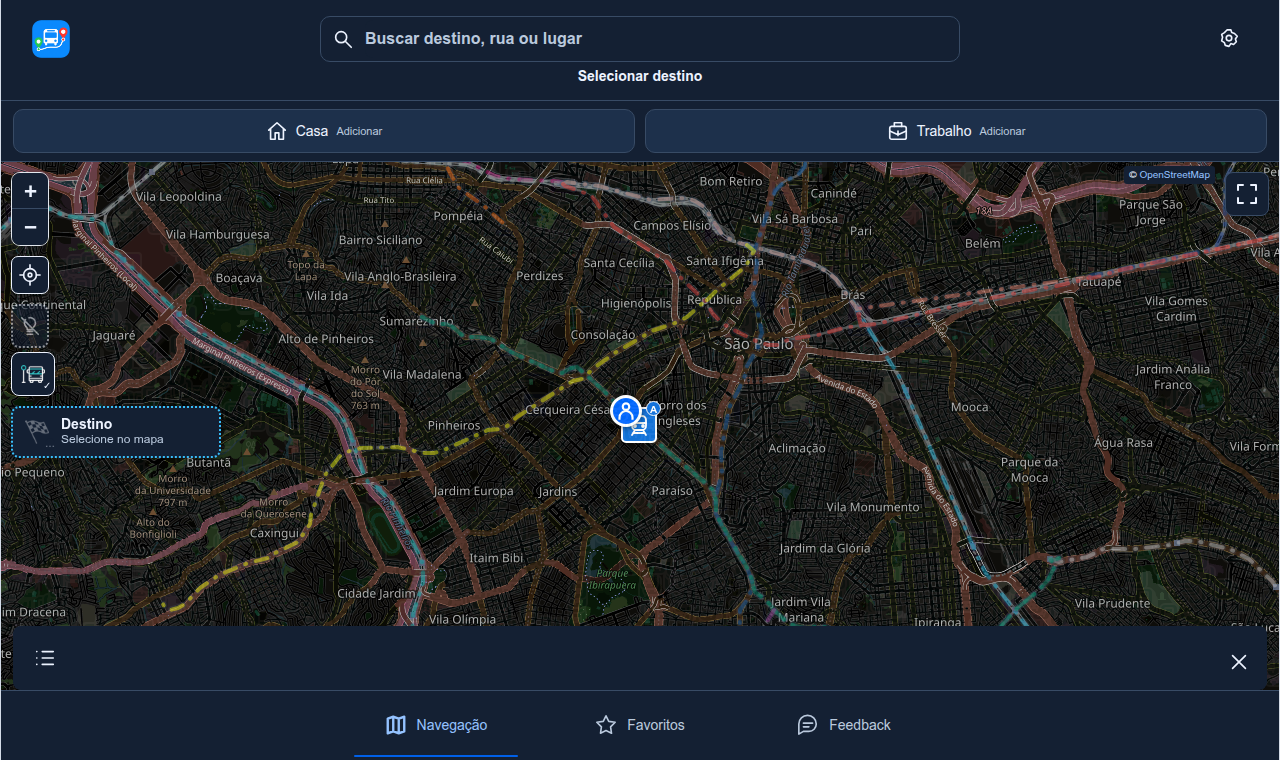
\includegraphics[width=\textwidth]{revisao-consistencia-2026-11-01/network-current.png}
\caption{Rede ferroviária e símbolos de estações antes da escolha do itinerário.}\label{fig:rede-ferroviaria-20261101}
\fonte{Captura local de 1 nov. 2026; roteiro capture\_final.cjs e hashes no manifesto da revisão.}
\end{figure}
\begin{figure}[H]
\centering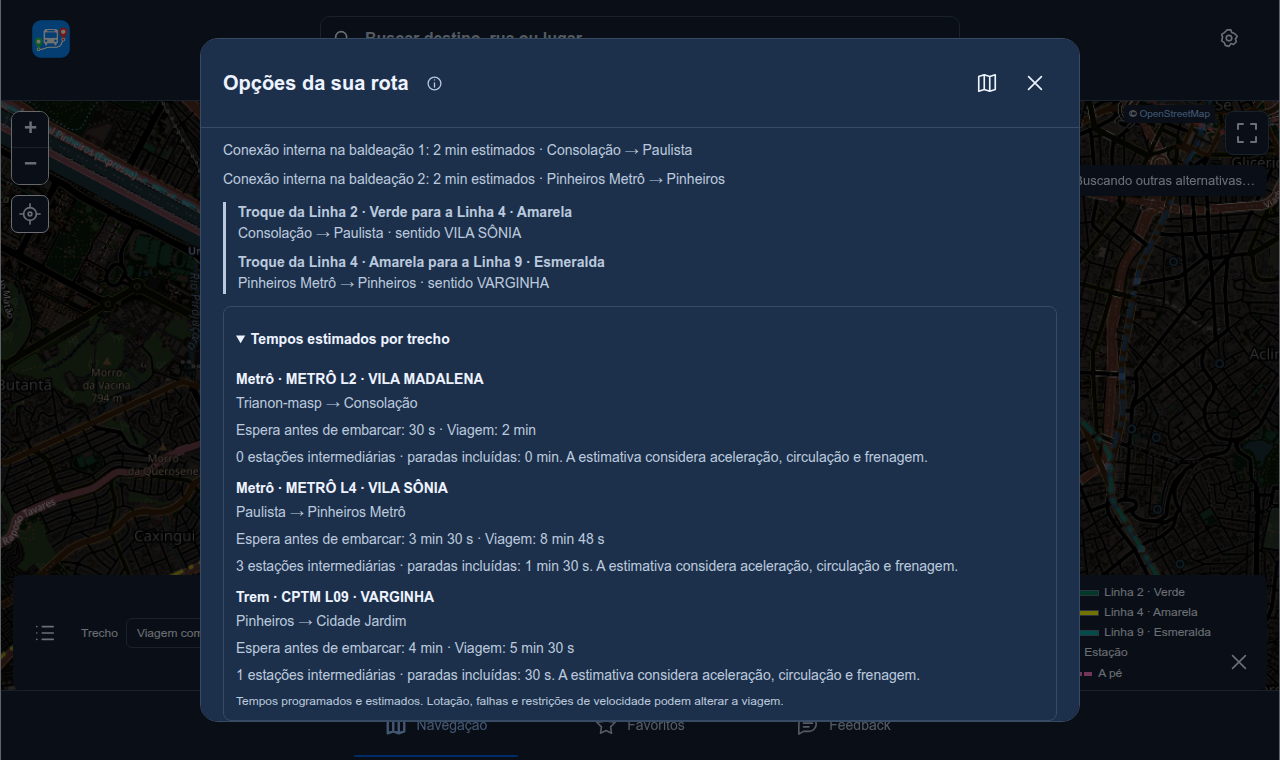
\includegraphics[width=\textwidth]{revisao-consistencia-2026-11-01/train-transfer-current.png}
\caption{Transferências Verde--Amarela--Esmeralda e decomposição das estimativas ferroviárias.}\label{fig:troca-ferroviaria-20261101}
\fonte{Mesma execução local; tempos de planejamento, sem previsão ferroviária em tempo real.}
\end{figure}

\subsection{Rastreabilidade}
As evidências estão no repositório de desenvolvimento: \nolinkurl{docs/coverage-audit-20261101.md}, \nolinkurl{docs/endpoint-audit-20261101.md}, \nolinkurl{docs/async-route-stream.md} e \nolinkurl{docs/async-performance-comparison.md}. O diretório \nolinkurl{artifacts/benchmarks/async-comparison-20261101/} preserva resultados individuais, comparação JSON, CSV pareado e validação das bases. O histórico de 28 de outubro a seguir conserva a estimativa de 226,47 GiB do desenho anterior; esse valor não corresponde ao tamanho final do banco compacto atual.


A conferência documental está em \nolinkurl{revisao-consistencia-2026-11-01/}, junto a este fonte. O CSV dos 477 casos preserva identificadores de paradas, grupos, custos e tempos, sem acessar telemetria pessoal. O manifesto retrospectivo registra hashes SHA-256 dos arquivos individuais de medição, scripts e evidências visuais, metadados dos bancos e o estado Git observado na auditoria. O HEAD de desenvolvimento observado foi \texttt{34a46f29}, com alterações locais; esse identificador sozinho não reproduz o código executado no teste. Não foi localizado no diretório do benchmark um manifesto contemporâneo completo que vincule cada execução a todos os fontes locais e à carga do equipamento.

O equipamento inspecionado nesta auditoria apresenta Intel Core i9-14900HX, 24 núcleos físicos e 32 processadores lógicos; o teste registrado utiliza 32 processos, não 32 núcleos físicos. O instrumento mantém o GTFS carregado, esvazia o cache de respostas a cada caso, recria os conjuntos de threads e aguarda o encerramento dos produtores fora do cronômetro da primeira rota. O cache do sistema operacional não foi isolado, impedindo classificar o resultado como ensaio controlado de cache frio. Os registros de execução são de 1 de novembro; 3 de novembro às 02h, 08h e 14h são instantes simulados de partida, não datas de coleta.

Os bancos foram identificados por assinatura, tamanho e data de modificação: GTFS importado em 6 de outubro, versão 2 da representação compacta e modelo ferroviário \texttt{rail-1}. As etapas-base concluídas são 0 e 1; as expansões completam vagas com limite de 8 e depois 12 unidades de um terço, preservando cinco alternativas e mínimo mais uma unidade de custo. Esses parâmetros, os limites pedestres e as assinaturas dos kernels constam do manifesto. A revisão não recalculou hash integral do banco de 88,44 GiB, não modificou dados brutos e não executou nova materialização ou benchmark. As lacunas de rastreabilidade são explicitadas, sem reconstruir retrospectivamente condições não registradas.
